\section{Easom Function}
\label{sec:app:test:easom}

  The \emph{Easom function} is a well-known unimodal benchmark function employed 
  in the evaluation of optimization algorithms.
  It gains its name from Charles Easom and is distinctively recognized by its 
  `needle'-like global minimum.
  This feature presents a demanding task for optimization algorithms due to its
  confined optimal search space.

  \begin{definition}[Easom Function]
    \label{def:app:test:easom}
    The \emph{Easom function}, defined for \(f: [-100,\,100]^2 \rightarrow 
    \mathbb{R}\), is formally expressed as:

    \begin{equation}
      \label{eq:app:test:easom}
      f(x,\, y) = -\cos(x)\cos(y)\exp\left(-((x-\pi)^2+(y-\pi)^2)\right)
    \end{equation}
    
    Here, \(x\) and \(y\) constitute the decision variables.
  \end{definition}

  The global minimum of the Easom function is situated at the coordinates 
  \(f(\pi,\, \pi) = -1\).

  The intricate structure and narrow optimal space of the Easom function are
  clearly revealed in its contour and surface plots. 

  \begin{figure}[ht!]
    \centering
    \begin{subfigure}[b]{0.45\textwidth}
      \centering
      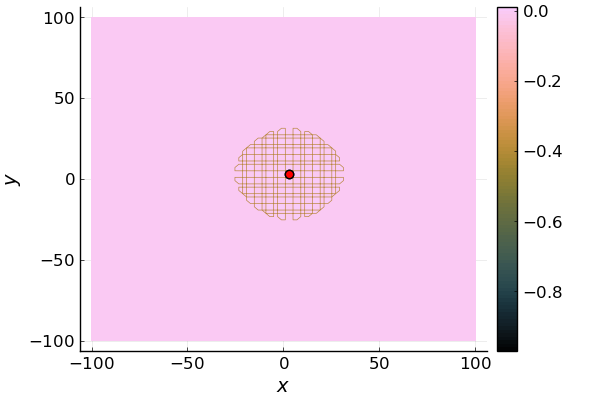
\includegraphics[width=\textwidth]{img/test_functions/easom_contour.png}
      \caption{
        Contour plot of the Easom function with the global minimum represented by 
        the red dot
      }
      \label{fig:app:test:easom:contour}
    \end{subfigure}
    \hfill
    \begin{subfigure}[b]{0.45\textwidth}
      \centering
      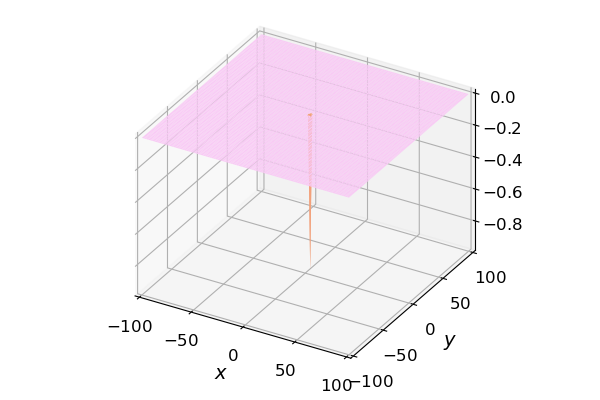
\includegraphics[width=\textwidth]{img/test_functions/easom_surface.png}
      \caption{Surface plot of the Easom function}
      \label{fig:app:test:easom:surface}
    \end{subfigure}
    \begin{subfigure}[b]{0.45\textwidth}
      \centering
      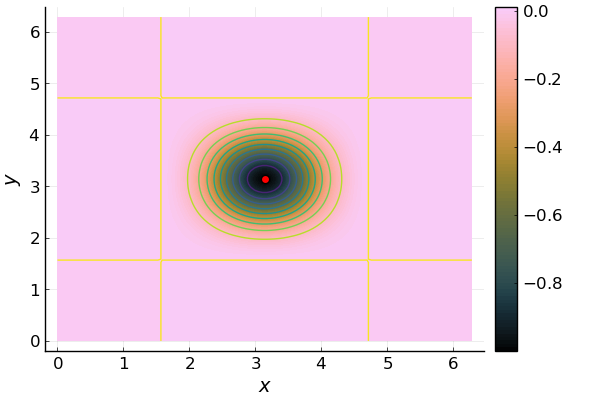
\includegraphics[width=\textwidth]
        {img/test_functions/easom_contour_closeup.png}
      \caption{
        Contour plot of the Easom function in the vicinity of the global minimum,
        \([0,\, 2\pi]\).
      }
      \label{fig:app:test:easom:contour:closeup}
    \end{subfigure}
    \hfill
    \begin{subfigure}[b]{0.45\textwidth}
      \centering
      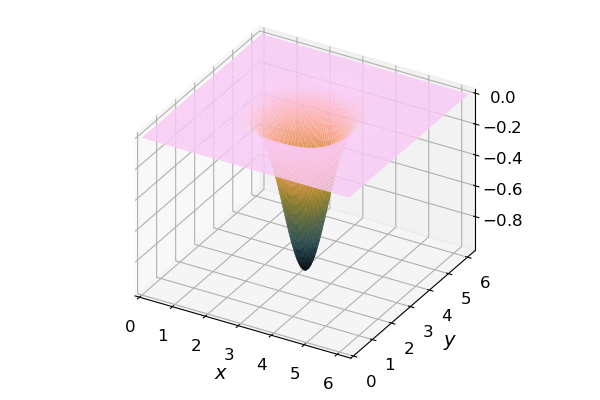
\includegraphics[width=\textwidth]
        {img/test_functions/easom_surface_closeup.png}
      \caption{
        Surface plot of the Easom function in the vicinity of the global minimum,
        \([0,\, 2\pi]\).
      }
      \label{fig:app:test:easom:surface:closeup}
    \end{subfigure}
    \caption{Contour and surface visualizations of the Easom function}
    \label{fig:app:test:easom}
  \end{figure}
